\documentclass[a4paper,11pt,dvipsnames,twoside,openright]{memoir} 	% Openright aabner kapitler paa hoejresider (openany begge)

%%%% PACKAGES %%%%

% ¤¤ Oversaettelse og tegnsaetning ¤¤ %
\usepackage[utf8]{inputenc}					% Input-indkodning af tegnsaet (UTF8)
\usepackage[english]{babel}					% Dokumentets sprog
\usepackage[T1]{fontenc}					% Output-indkodning af tegnsaet (T1)
\usepackage{lmodern}						% Noget jeg selv har indsat, fordi det ellers ikke virkede
\usepackage{ragged2e,anyfontsize}			% Justering af elementer
%\usepackage{fixltx2e}						% Retter forskellige fejl i LaTeX-kernen
																			
% ¤¤ Figurer og tabeller (floats) ¤¤ %
\usepackage{graphicx} 						% Haandtering af eksterne billeder (JPG, PNG, EPS, PDF)
%\usepackage{eso-pic}						% Tilfoej billedekommandoer paa hver side
\usepackage{wrapfig}						% Indsaettelse af figurer omsvoebt af tekst. \begin{wrapfigure}{Placering}{Stoerrelse}
\usepackage{multirow}                		% Fletning af raekker og kolonner (\multicolumn og \multirow)
\usepackage{multicol}         	        	% Muliggoer output i spalter
\usepackage{rotating}						% Rotation af tekst med \begin{sideways}...\end{sideways}
\usepackage{colortbl} 						% Farver i tabeller (fx \columncolor og \rowcolor)
\usepackage{xcolor}							% Definer farver med \definecolor. Se mere: http://en.wikibooks.org/wiki/LaTeX/Colors
\usepackage{flafter}						% Soerger for at floats ikke optraeder i teksten foer deres reference
\let\newfloat\relax 						% Justering mellem float-pakken og memoir
\usepackage{float}							% Muliggoer eksakt placering af floats, f.eks. \begin{figure}[H]

% ¤¤ Matematik mm. ¤¤
\usepackage{amsmath,amssymb,stmaryrd} 		% Avancerede matematik-udvidelser
\usepackage{mathtools}						% Andre matematik- og tegnudvidelser
\usepackage{textcomp}                 		% Symbol-udvidelser (f.eks. promille-tegn med \textperthousand )
\usepackage{rsphrase}						% Kemi-pakke til RS-saetninger, f.eks. \rsphrase{R1}
\usepackage[version=3]{mhchem} 				% Kemi-pakke til flot og let notation af formler, f.eks. \ce{Fe2O3}
\usepackage{siunitx}						% Flot og konsistent praesentation af tal og enheder med \si{enhed} og \SI{tal}{enhed}
\sisetup{output-decimal-marker = {,}}		% Opsaetning af \SI (DE for komma som decimalseparator) 

% ¤¤ Referencer og kilder ¤¤ %
\usepackage[english]{varioref}				% Muliggoer bl.a. krydshenvisninger med sidetal (\vref)
\usepackage{natbib}
% Udvidelse med naturvidenskabelige citationsmodeller
%\usepackage{xr}							% Referencer til eksternt dokument med \externaldocument{<NAVN>}
%\usepackage{glossaries}					% Terminologi- eller symbolliste (se mere i Daleifs Latex-bog)

%indsat af jeno
\usepackage{paralist}
%indsat af Andreas
%\DeclareUnicodeCharacter{00A0}{~}

% ¤¤ Misc. ¤¤ %
\usepackage{listings}						% Placer kildekode i dokumentet med \begin{lstlisting}...\end{lstlisting}
\usepackage{lipsum}							% Dummy text \lipsum[..]
\usepackage[shortlabels]{enumitem}			% Muliggoer enkelt konfiguration af lister
\usepackage{pdfpages}						% Goer det muligt at inkludere pdf-dokumenter med kommandoen \includepdf[pages={x-y}]{fil.pdf}	
\pdfminorversion=6					% Muliggoer inkludering af pdf dokumenter, af version 1.6 og hoejere - Andreas: Jeg aendrede en gang pdfoptionpdfminorversion -> pdfminorversion, saa hvis noget en gang gaar galt, saa kunne det vaere derfor
\pretolerance=2500 							% Justering af afstand mellem ord (hoejt tal, mindre orddeling og mere luft mellem ord)

% Kommentarer og rettelser med \fxnote. Med 'final' i stedet for 'draft' udloeser hver note en error i den faerdige rapport.
\usepackage[footnote,draft,english,silent,nomargin]{fixme}		


%%%% CUSTOM SETTINGS %%%%

% ¤¤ Marginer ¤¤ %
\setlrmarginsandblock{3.5cm}{2.5cm}{*}		% \setlrmarginsandblock{Indbinding}{Kant}{Ratio}
\setulmarginsandblock{2.5cm}{3.0cm}{*}		% \setulmarginsandblock{Top}{Bund}{Ratio}
\checkandfixthelayout 						% Oversaetter vaerdier til brug for andre pakker

%	¤¤ Afsnitsformatering ¤¤ %
\setlength{\parindent}{0mm}           		% Stoerrelse af indryk
\setlength{\parskip}{3mm}          			% Afstand mellem afsnit ved brug af double Enter
\linespread{1,1}							% Linie afstand

% ¤¤ Litteraturlisten ¤¤ %
\bibpunct[,]{[}{]}{;}{a}{,}{,} 				% Definerer de 6 parametre ved Harvard henvisning (bl.a. parantestype og seperatortegn)
\bibliographystyle{bibtex/harvard}			% Udseende af litteraturlisten.

% ¤¤ Indholdsfortegnelse ¤¤ %
\setsecnumdepth{subsection}		 			% Dybden af nummerede overkrifter (part/chapter/section/subsection)
\maxsecnumdepth{subsection}					% Dokumentklassens graense for nummereringsdybde
\settocdepth{section} 					% Dybden af indholdsfortegnelsen

% ¤¤ Lister ¤¤ %
\setlist{
  topsep=0pt,								% Vertikal afstand mellem tekst og listen
  itemsep=-1ex,								% Vertikal afstand mellem items
} 

% ¤¤ Visuelle referencer ¤¤ %
\usepackage[colorlinks]{hyperref}			% Danner klikbare referencer (hyperlinks) i dokumentet.
\hypersetup{colorlinks = true,				% Opsaetning af farvede hyperlinks (interne links, citeringer og URL)
    linkcolor = black,
    citecolor = black,
    urlcolor = black
}

% ¤¤ Opsaetning af figur- og tabeltekst ¤¤ %
\captionnamefont{\small\bfseries\itshape}	% Opsaetning af tekstdelen ('Figur' eller 'Tabel')
\captiontitlefont{\small}					% Opsaetning af nummerering
\captiondelim{. }							% Seperator mellem nummerering og figurtekst
\hangcaption								% Venstrejusterer flere-liniers figurtekst under hinanden
\captionwidth{\linewidth}					% Bredden af figurteksten
\setlength{\belowcaptionskip}{0pt}			% Afstand under figurteksten
		
% ¤¤ Opsaetning af listings ¤¤ %

\definecolor{commentGreen}{RGB}{34,139,24}
\definecolor{stringPurple}{RGB}{208,76,239}

\lstset{language=Matlab,					% Sprog
	basicstyle=\ttfamily\scriptsize,		% Opsaetning af teksten
	keywords={for,if,while,else,elseif,		% Noegleord at fremhaeve
			  end,break,return,case,
			  switch,function},
	keywordstyle=\color{blue},				% Opsaetning af noegleord
	commentstyle=\color{commentGreen},		% Opsaetning af kommentarer
	stringstyle=\color{stringPurple},		% Opsaetning af strenge
	showstringspaces=false,					% Mellemrum i strenge enten vist eller blanke
	numbers=left, numberstyle=\tiny,		% Linjenumre
	extendedchars=true, 					% Tillader specielle karakterer
	columns=flexible,						% Kolonnejustering
	breaklines, breakatwhitespace=true,		% Bryd lange linjer
}


%This is the code for including Python

\definecolor{maroon}{cmyk}{0, 0.87, 0.68, 0.32}
\definecolor{halfgray}{gray}{0.55}
\definecolor{ipython_frame}{RGB}{207, 207, 207}
\definecolor{ipython_bg}{RGB}{247, 247, 247}
\definecolor{ipython_red}{RGB}{186, 33, 33}
\definecolor{ipython_green}{RGB}{0, 128, 0}
\definecolor{ipython_cyan}{RGB}{64, 128, 128}
\definecolor{ipython_purple}{RGB}{170, 34, 255}

%% Python definition (c) 1998 Michael Weber
%% Additional definitions (2013) Alexis Dimitriadis
%% modified by me (should not have empty lines)
%%
\lstdefinelanguage{iPython}{
    morekeywords={access,and,break,class,continue,def,del,elif,else,except,exec,finally,for,from,global,if,import,in,is,lambda,not,or,pass,print,raise,return,try,while},%
    %
    % Built-ins
    morekeywords=[2]{abs,all,any,basestring,bin,bool,bytearray,callable,chr,classmethod,cmp,compile,complex,delattr,dict,dir,divmod,enumerate,eval,execfile,file,filter,float,format,frozenset,getattr,globals,hasattr,hash,help,hex,id,input,int,isinstance,issubclass,iter,len,list,locals,long,map,max,memoryview,min,next,object,oct,open,ord,pow,property,range,raw_input,reduce,reload,repr,reversed,round,set,setattr,slice,sorted,staticmethod,str,sum,super,tuple,type,unichr,unicode,vars,xrange,zip,apply,buffer,coerce,intern},%
    %
    sensitive=true,%
    morecomment=[l]\#,%
    morestring=[b]',%
    morestring=[b]",%
    %
    morestring=[s]{'''}{'''},% used for documentation text (mulitiline strings)
    morestring=[s]{"""}{"""},% added by Philipp Matthias Hahn
    %
    morestring=[s]{r'}{'},% `raw' strings
    morestring=[s]{r"}{"},%
    morestring=[s]{r'''}{'''},%
    morestring=[s]{r"""}{"""},%
    morestring=[s]{u'}{'},% unicode strings
    morestring=[s]{u"}{"},%
    morestring=[s]{u'''}{'''},%
    morestring=[s]{u"""}{"""},%
    %
    % {replace}{replacement}{lenght of replace}
    % *{-}{-}{1} will not replace in comments and so on
    literate=
    {á}{{\'a}}1 {é}{{\'e}}1 {í}{{\'i}}1 {ó}{{\'o}}1 {ú}{{\'u}}1
    {Á}{{\'A}}1 {É}{{\'E}}1 {Í}{{\'I}}1 {Ó}{{\'O}}1 {Ú}{{\'U}}1
    {à}{{\`a}}1 {è}{{\`e}}1 {ì}{{\`i}}1 {ò}{{\`o}}1 {ù}{{\`u}}1
    {À}{{\`A}}1 {È}{{\'E}}1 {Ì}{{\`I}}1 {Ò}{{\`O}}1 {Ù}{{\`U}}1
    {ä}{{\"a}}1 {ë}{{\"e}}1 {ï}{{\"i}}1 {ö}{{\"o}}1 {ü}{{\"u}}1
    {Ä}{{\"A}}1 {Ë}{{\"E}}1 {Ï}{{\"I}}1 {Ö}{{\"O}}1 {Ü}{{\"U}}1
    {â}{{\^a}}1 {ê}{{\^e}}1 {î}{{\^i}}1 {ô}{{\^o}}1 {û}{{\^u}}1
    {Â}{{\^A}}1 {Ê}{{\^E}}1 {Î}{{\^I}}1 {Ô}{{\^O}}1 {Û}{{\^U}}1
    {œ}{{\oe}}1 {Œ}{{\OE}}1 {æ}{{\ae}}1 {Æ}{{\AE}}1 {ß}{{\ss}}1
    {ç}{{\c c}}1 {Ç}{{\c C}}1 {ø}{{\o}}1 {å}{{\r a}}1 {Å}{{\r A}}1
    {€}{{\EUR}}1 {£}{{\pounds}}1
    %
    {^}{{{\color{ipython_purple}\^{}}}}1
    {=}{{{\color{ipython_purple}=}}}1
    %
    {+}{{{\color{ipython_purple}+}}}1
    {*}{{{\color{ipython_purple}$^\ast$}}}1
    {/}{{{\color{ipython_purple}/}}}1
    %
    {+=}{{{+=}}}1
    {-=}{{{-=}}}1
    {*=}{{{$^\ast$=}}}1
    {/=}{{{/=}}}1,
    literate=
    *{-}{{{\color{ipython_purple}-}}}1
     {?}{{{\color{ipython_purple}?}}}1,
    %
    identifierstyle=\color{black}\ttfamily,
    commentstyle=\color{ipython_cyan}\ttfamily,
    stringstyle=\color{ipython_red}\ttfamily,
    keepspaces=true,
    showspaces=false,
    showstringspaces=false,
    %
    rulecolor=\color{ipython_frame},
    frame=single,
    frameround={t}{t}{t}{t},
    framexleftmargin=6mm,
    breaklines=true,                 
    captionpos=b, 
    numbers=left,
    numberstyle=\tiny\color{halfgray},
    %
    %
    backgroundcolor=\color{ipython_bg},
    %   extendedchars=true,
    basicstyle=\scriptsize,
    keywordstyle=\color{ipython_green}\ttfamily,
}

\lstdefinelanguage{JavaScript}{
	morekeywords={typeof, new, true, false, catch, function, return, null, catch, switch, var, if, in, while, do, else, case, break},
	morecomment=[s]{/*}{*/},
	morecomment=[l]//,
	morestring=[b]",
	morestring=[b]',
	identifierstyle=\color{black}\ttfamily,
	commentstyle=\color{ipython_red}\ttfamily,
	stringstyle=\color{ipython_green}\ttfamily,
	rulecolor=\color{ipython_frame},
	frame=single,
	frameround={t}{t}{t}{t},
	framexleftmargin=6mm,
	breaklines=true,                 
	captionpos=b, 
	numbers=left,
	numberstyle=\tiny\color{halfgray},
	%
	%
	backgroundcolor=\color{ipython_bg},
	%   extendedchars=true,
	basicstyle=\scriptsize,
	keywordstyle=\color{blue}\ttfamily,
}

\lstdefinelanguage{CSS}{
	keywords={color,background-image:,margin,padding,font,weight,display,position,top,left,right,bottom,list,style,border,size,white,space,min,width, transition:, transform:, transition-property, transition-duration, transition-timing-function},	
	sensitive=true,
	morecomment=[l]{//},
	morecomment=[s]{/*}{*/},
	morestring=[b]',
	morestring=[b]",
	alsoletter={:},
	alsodigit={-},
	identifierstyle=\color{black}\ttfamily,
	commentstyle=\color{ipython_red}\ttfamily,
	stringstyle=\color{ipython_green}\ttfamily,
	rulecolor=\color{ipython_frame},
	frame=single,
	frameround={t}{t}{t}{t},
	framexleftmargin=6mm,
	breaklines=true,                 
	captionpos=b, 
	numbers=left,
	numberstyle=\tiny\color{halfgray},
	%
	%
	backgroundcolor=\color{ipython_bg},
	%   extendedchars=true,
	basicstyle=\scriptsize,
	keywordstyle=\color{blue}\ttfamily,
}

\lstdefinelanguage{HTML5}{
	language=html,
	sensitive=true,	
	alsoletter={<>=-},	
	morecomment=[s]{<!-}{-->},
	tag=[s],
	otherkeywords={
		% General
		>,
		% Standard tags
		<!DOCTYPE,
		</html, <html, <head, <title, </title, <style, </style, <link, </head, <meta, />,
		% body
		</body, <body,
		% Divs
		</div, <div, </div>, 
		% Paragraphs
		</p, <p, </p>,
		% scripts
		</script, <script,
		% More tags...
		<canvas, /canvas>, <svg, <rect, <animateTransform, </rect>, </svg>, <video, <source, <iframe, </iframe>, </video>, <image, </image>, <header, </header, <article, </article
	},
	identifierstyle=\color{black}\ttfamily,
	commentstyle=\color{ipython_red}\ttfamily,
	stringstyle=\color{ipython_green}\ttfamily,
	rulecolor=\color{ipython_frame},
	frame=single,
	frameround={t}{t}{t}{t},
	framexleftmargin=6mm,
	breaklines=true,                 
	captionpos=b, 
	numbers=left,
	numberstyle=\tiny\color{halfgray},
	%
	%
	backgroundcolor=\color{ipython_bg},
	%   extendedchars=true,
	basicstyle=\scriptsize,
	keywordstyle=\color{blue}\ttfamily,
	ndkeywords={
		% General
		=,
		% HTML attributes
		charset=, src=, id=, width=, height=, style=, type=, rel=, href=,
		% SVG attributes
		fill=, attributeName=, begin=, dur=, from=, to=, poster=, controls=, x=, y=, repeatCount=, xlink:href=,
		% properties
		margin:, padding:, background-image:, border:, top:, left:, position:, width:, height:, margin-top:, margin-bottom:, font-size:, line-height:,
		% CSS3 properties
		transform:, -moz-transform:, -webkit-transform:,
		animation:, -webkit-animation:,
		transition:,  transition-duration:, transition-property:, transition-timing-function:,
	}
}

%To here

% ¤¤ Navngivning ¤¤ %
\addto\captionsdanish{
	\renewcommand\appendixname{Bilag}
	\renewcommand\contentsname{Indholdsfortegnelse}	
	\renewcommand\appendixpagename{Appendix}
	\renewcommand\appendixtocname{Appendix}
	\renewcommand\cftchaptername{\chaptername~}				% Skriver "Kapitel" foran kapitlerne i indholdsfortegnelsen
	\renewcommand\cftappendixname{\appendixname~}			% Skriver "Appendiks" foran appendiks i indholdsfortegnelsen
}

% ¤¤ Kapiteludssende ¤¤ %
\definecolor{numbercolor}{gray}{0.7}		% Definerer en farve til brug til kapiteludseende
\newif\ifchapternonum

\makechapterstyle{jenor}{					% Definerer kapiteludseende frem til ...
  \renewcommand\beforechapskip{0pt}
  \renewcommand\printchaptername{}
  \renewcommand\printchapternum{}
  \renewcommand\printchapternonum{\chapternonumtrue}
  \renewcommand\chaptitlefont{\fontfamily{pbk}\fontseries{db}\fontshape{n}\fontsize{25}{35}\selectfont\raggedleft}
  \renewcommand\chapnumfont{\fontfamily{pbk}\fontseries{m}\fontshape{n}\fontsize{1in}{0in}\selectfont\color{numbercolor}}
  \renewcommand\printchaptertitle[1]{%
    \noindent
    \ifchapternonum
    \begin{tabularx}{\textwidth}{X}
    {\let\\\newline\chaptitlefont ##1\par} 
    \end{tabularx}
    \par\vskip-2.5mm\hrule
    \else
    \begin{tabularx}{\textwidth}{Xl}
    {\parbox[b]{\linewidth}{\chaptitlefont ##1}} & \raisebox{-15pt}{\chapnumfont \thechapter}
    \end{tabularx}
    \par\vskip2mm\hrule
    \fi
  }
}											% ... her

\chapterstyle{jenor}						% Valg af kapiteludseende - Google 'memoir chapter styles' for alternativer

% ¤¤ Sidehoved ¤¤ %

\makepagestyle{AAU}							% Definerer sidehoved og sidefod udseende frem til ...
\makepsmarks{AAU}{%
	\createmark{chapter}{left}{shownumber}{}{. \ }
	\createmark{section}{right}{shownumber}{}{. \ }
	\createplainmark{toc}{both}{\contentsname}
	\createplainmark{lof}{both}{\listfigurename}
	\createplainmark{lot}{both}{\listtablename}
	\createplainmark{bib}{both}{\bibname}
	\createplainmark{index}{both}{\indexname}
	\createplainmark{glossary}{both}{\glossaryname}
}
\nouppercaseheads											% Ingen Caps oenskes

\makeevenhead{AAU}{Andreas Gram Riisgaard}{}{\leftmark}				% Definerer lige siders sidehoved (\makeevenhead{Navn}{Venstre}{Center}{Hoejre})
\makeoddhead{AAU}{\rightmark}{}{Aalborg University}		% Definerer ulige siders sidehoved (\makeoddhead{Navn}{Venstre}{Center}{Hoejre})
\makeevenfoot{AAU}{\thepage}{}{}							% Definerer lige siders sidefod (\makeevenfoot{Navn}{Venstre}{Center}{Hoejre})
\makeoddfoot{AAU}{}{}{\thepage}								% Definerer ulige siders sidefod (\makeoddfoot{Navn}{Venstre}{Center}{Hoejre})
\makeheadrule{AAU}{\textwidth}{0.5pt}						% Tilfoejer en streg under sidehovedets indhold
\makefootrule{AAU}{\textwidth}{0.5pt}{1mm}					% Tilfoejer en streg under sidefodens indhold

\copypagestyle{AAUchap}{AAU}								% Sidehoved for kapitelsider defineres som standardsider, men med blank sidehoved
\makeoddhead{AAUchap}{}{}{}
\makeevenhead{AAUchap}{}{}{}
\makeheadrule{AAUchap}{\textwidth}{0pt}
\aliaspagestyle{chapter}{AAUchap}							% Den ny style vaelges til at gaelde for chapters
															% ... her
															
\pagestyle{AAU}												% Valg af sidehoved og sidefod


%%%% CUSTOM COMMANDS %%%%

% ¤¤ Billede hack ¤¤ %
\newcommand{\figur}[4]{
		\begin{figure}[H] \centering
			\includegraphics[width=#1\textwidth]{Pictures/#2}
			\caption{#3}\label{#4}
		\end{figure} 
}

% ¤¤ Specielle tegn ¤¤ %
\newcommand{\decC}{^{\circ}\text{C}}
\newcommand{\dec}{^{\circ}}
\newcommand{\m}{\cdot}


%%%% ORDDELING %%%%

\hyphenation{}


%Egne tilføjelser!!!
%En figurtekst til flere billeder

% %Det her er linjeopdeling
% \usepackage{lineno}
% \usepackage{dcolumn}   % needed for some tables
% \usepackage{bm}        % for math
% \usepackage{amssymb}   % for math


\usepackage{microtype}
%\usepackage{grffile}
\usepackage{cite}
\usepackage{paralist}
\usepackage[ampersand]{easylist}
\usepackage{etoolbox}
\usepackage{titlesec}
\usepackage[section]{placeins}
%\usepackage{caption}
\usepackage{subfig}
\usepackage{adjustbox}
\usepackage{array}
\usepackage{rotating}
\usepackage[footnote,draft,english,silent,nomargin]{fixme}

\newcolumntype{R}[2]{%
   >{\adjustbox{angle=#1,lap=\width-(#2)}\bgroup}%
    l%
    <{\egroup}%
}
\newcommand*\rot{\multicolumn{1}{R{90}{1em}}}% no optional argument here, please!
	
										% Preamble indlaeses
\raggedbottom													% Soerger for at LaTeX ikke "straekker" teksten

%\includeonly{file1,file2}										% Inkluder kun specifikke filer (kommasepareret liste)

\begin{document}												% Starter dokumentet - obligatorisk


\thispagestyle{empty}

\begin{center}
\textsc{\LARGE Aalborg University}\\%[0.5cm]	
\textsc{\Large Geoinformatics}\\[1.cm]
\end{center}

\begin{figure} [H]
	\centering
	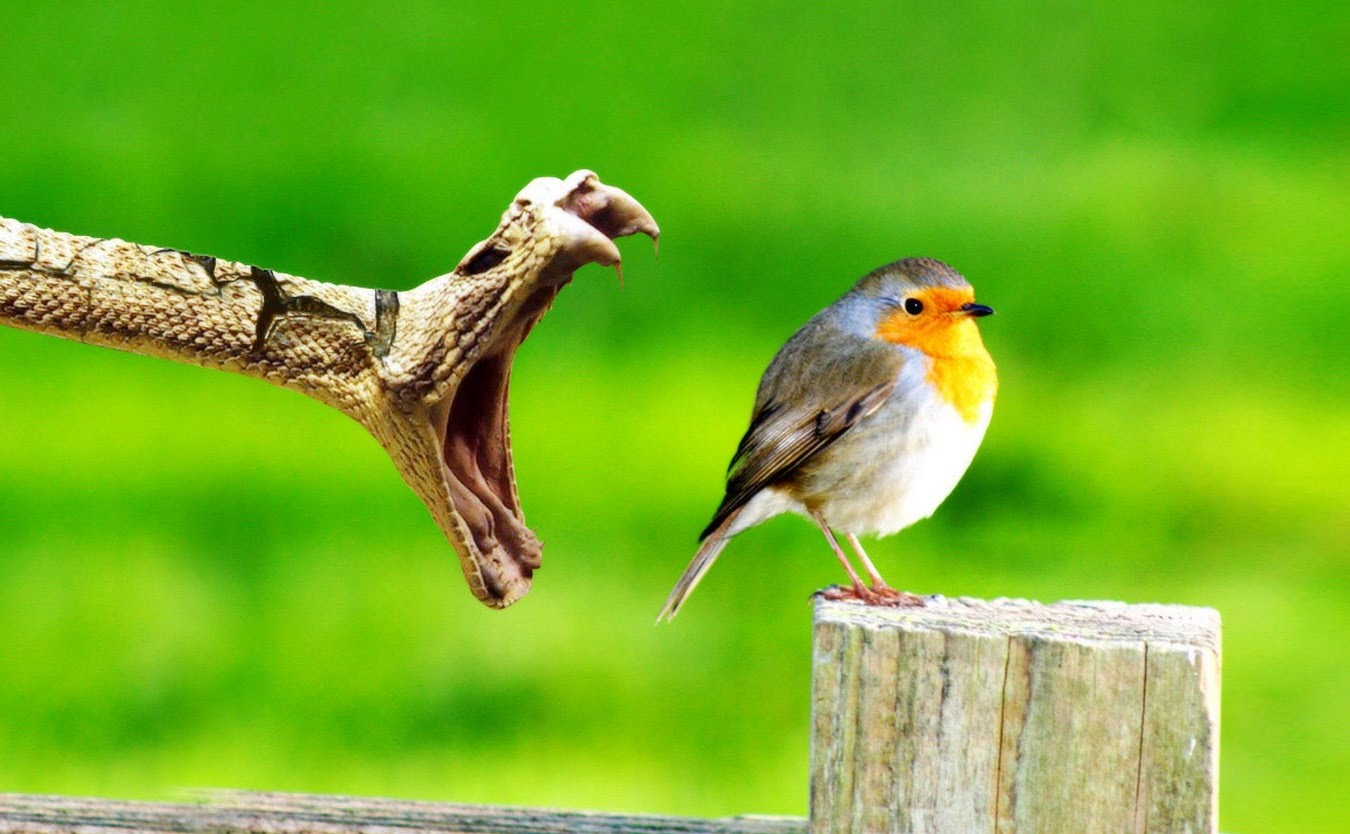
\includegraphics[width=1\textwidth]{Pictures/Example.jpg}	
	\label{forside}
\end{figure}

\vfill
\begin{center}
{ \huge \bfseries {Project titel - edit this in Formalia/FrontPage}}\\[0.2cm]
%{\large \bfseries {}}
\end{center}

% Author and supervisor
\begin{tabularx}{\textwidth}{l X r}
	\hline
	\emph{Authors:} & & \emph{Supervisors:}\\
	Name 1	&	 &	 Supervisor 1 \\
	Name 2     	&	 &	Supervisor 2  \\
	Name 3		\\
	Name 4       \\
	\hline
\end{tabularx}

\vfill

% Bottom of the page
{\large January 2019}

\frontmatter

% \begin{figure}[H]
% 	\centering
% 	\includegraphics[width=0.5\textwidth]{billeder/Matrikelkort.jpg}
% 	\caption{Kort over hvilke matrikler, der henholdsvis er under kommunens og skolens ansvar. Udarbejdet af projektgruppen på baggrund af data fra \citep{Skolematrikel}.}
% 	\label{Matrikelkort}
% \end{figure}
\frontmatter													% Forindhold - nummereres med romertal


\cleardoublepage												% Indsaetter tom side, saa naeste kapitel starter paa hoejre side (hvis noedvendigt)
\pagenumbering{roman}
\setcounter{page}{1}

% \begin{minipage}[t]{0.48\textwidth}
% \vspace*{-25pt}			%\vspace*{-9pt}
% %\includegraphics[height=4cm]{billeder/aau_logo}
% \end{minipage}
% \hfill
% \begin{minipage}[t]{0.48\textwidth}
% {\small 
% \textbf{Tredje Studieår v/ Det Teknisk-}\\
% \textbf{Naturvidenskabelige Fakultet}  \\
% By-, Energi- og Miljøplanlægning\\
% Rendsburggade 6 \\
% 9000 Aalborg \\}
% \end{minipage}

\vspace*{1cm}

\begin{minipage}[t]{0.48\textwidth}
\textbf{Titel:} \\[5pt]\hspace{2ex}
Visualizing and comparing population 
projection rasters

\vspace*{1cm}

\textbf{Projekt:} \\[5pt]\bigskip\hspace{2ex}
Thesis project

\textbf{Project Period:} \\[5pt]\bigskip\hspace{2ex}
February 2020 - June 2020

\textbf{Author:} \\[5pt]\hspace*{2ex}
Andreas Gram Riisgaard 
\\\bigskip\hspace{2ex}


\textbf{Supervisor:} \\[5pt]\hspace*{2ex}
Carsten Kessler \\\bigskip\hspace{2ex}



%\vspace*{1cm}

\textbf{Number of pages:} 71 \\
\textbf{Number of annexes:} 2 \\ 
\textbf{Afsluttet:} 4-6-2020
 
\end{minipage}
\hfill
\begin{minipage}[t]{0.8\textwidth}%483
 \textbf{Abstract:} \\[3pt]
 \fbox{\parbox{8cm}{\bigskip

In this thesis project an interactive tool for visual comparison of raster datasets have been developed using population projections as a case. 

To develop a tool able to enable such comparisons it is important to know how population projections should be visualized and which functionalities are important for the tool. There is a technical challenge in visualizing large raster datasets, while still maintaining a responsive user experience.

The conventions for visualization of population projections was explored through a literature review. A quantitative sequential dataset like a population projection should be colored, so that the areas with least population is colored in a lighter color, than the more densely populated areas. 

The functionalities for the tool was determined by comparing with another interactive map. It was decided to have two maps showing different population projections. The maps can be navigated either by panning and zooming or using a search bar. 

To ensure a responsive user experience the raster was not loaded into the tool in its entirety. Instead it was divided into smaller tiles, which got loaded based on the extent of the map. These tiles were then colored on the client.

The tool was created as an Openlayers map displaying tiles, which was created with a modified version of the python program gdal2tiles.
While the user experience is responsive while using the map the creation of tiles is time consuming. The tool could therefore be improved in the future by using cloud optimized geotiffs instead of tiles.
\bigskip}}
\end{minipage}

\cleardoublepage
\chapter{Preface} 
This is edited in the file Formalia/Preface

\cleardoublepage

%%%% Indholdsfortegnelse (TOC) %%%%

\phantomsection													% Kunstigt afsnit, som hyperlinks kan 'holde fast i'
\pdfbookmark[0]{Indholdsfortegnelse}{indhold}					% Tildeler en klikbar bookmark til den endelige PDF
\tableofcontents*												% Indholdsfortegnelsen (kaldet ToC) 

%\addtocontents{toc}{\protect\newpage}							% Fremtvinger sideskift i ToC hvis noedvendig (der hvor koden placeres)

\mainmatter														% Hovedindhold - nummereres fra side 1

%%%% Rapportindhold %%%% 										% Rapportindholdet boer IKKE indeholde broedtekst - KUN includede filer!

% Opdel evt. i passende afsnit for overblikkets skyld

\chapter{Introduction}

In 2019 the population in the world reached 7.7 billion people, which is an increase of one billion over the past twelve years. According to The United Nations Department of Economic and Social Affairs’ (UN DESA) median scenario the growth is expected to continue reaching 9.7 billon in 2050. \citep{UNDEASHightlights} 

To be able to adapt infrastructures to this population growth it is necessary to predict where these people will settle. While UN DESA provides this information on a national level \citep{NationalPop}, it is more ideal with a more nuanced picture, since most planning are based on local or regional scale spatial projections. \citep{WhyDetailedPop}

Other researchers (SEDAC, CISC) have used simulations to distribute the population within each country as raster layers. However due to the high resolution and/or small scales, visually comparing these raster datasets is a time-consuming task. The purpose of this project is to create a tool allowing fast and easy comparison of such raster datasets, focusing on the use case of population projections.

%Evt noget om at det vil være ekstra interessant at have områderne med stor vækst som case - tilføj her, hvis der skal argumenteres for en case senere

\section{Problem statement}

To explore the possibilities for creating such a comparison tool the following research question have been defined:

\textit{How can population rasters be visualized and compared efficiently and effectively?}

This broad main question will be answered by answering the following three subquestions:

\textbf{Which conventions exist for visualization of population projections?}

\textbf{Which functionalities are relevant for comparing different rasters?}

\textbf{How can a responsive user experience be ensured, when loading and visualizing large raster dataset?}


\section{Limitations}\label{Lim}

Determining relevant functionalities and the responsiveness would ideally have been done with user testing.  However it was determined that both the creation of the tool and a scientific approach to user testing would require too much time.
Therefore the tool creation got prioritised and other evaluation methods were chosen. This is expanded upon in section \ref{Eval}

\section{Target audience}\label{TA}

The target audience for this project is academical researchers. It is meant as a tool for these researcher to be able to quickly compare different population projections. 

This prototype of the tool have only been created for internal and individual use. It will therefore not be created with multiple users in mind and there will be no considerations for security.


The tool is also created with only computers in mind, so it will not be optimized for mobile. 

Alternative target audiences are being discussed in section x.

\section{Report structure}

\fxnote{ADD: quick overview of what the solution is going to be, what is population projections, SSP}

%The report have been divided into three parts. The first part is the literature review, which will address the first two subquestions and also present the two projections visualised in this project. Chapter x explores which conventions there exist for population projections, while the relevant functionalities for raster comparison are detailed in chapter x. Lastly chapter x will give an overview of the population projection SEDAC and CICS, which will be used as case for comparison.
%
%The second part is addressing the last subquestion. First there is a definition of how a "responsive user experience" has been defined. Then different methods of visualising raster datasets are being tested in chapter x. Based on these initial tests a method will chosen, which will be evaluated in the next section.
%
%The last part starts with a discussion in chapter x of the results of the previous part. This is then followed by the last two chapters x and x, which are the conclusion and future work.  

%Part I: Litterature review
%- Conventions, what are relevant functionalities, Explaining the two case projections
%
%Part II: Choice of method
%- Test of different methods 
%
%Part III: Discussion 

The report has been divided into three parts; design, development and evaluation.




In the design part the thought process behind the design of the solution is explained.
It starts with some background information about the case data in chapter x, raster formatting in chapter x and chapter x about how the raster data currently is being compared. 

\begin{figure} [H]
	\centering
	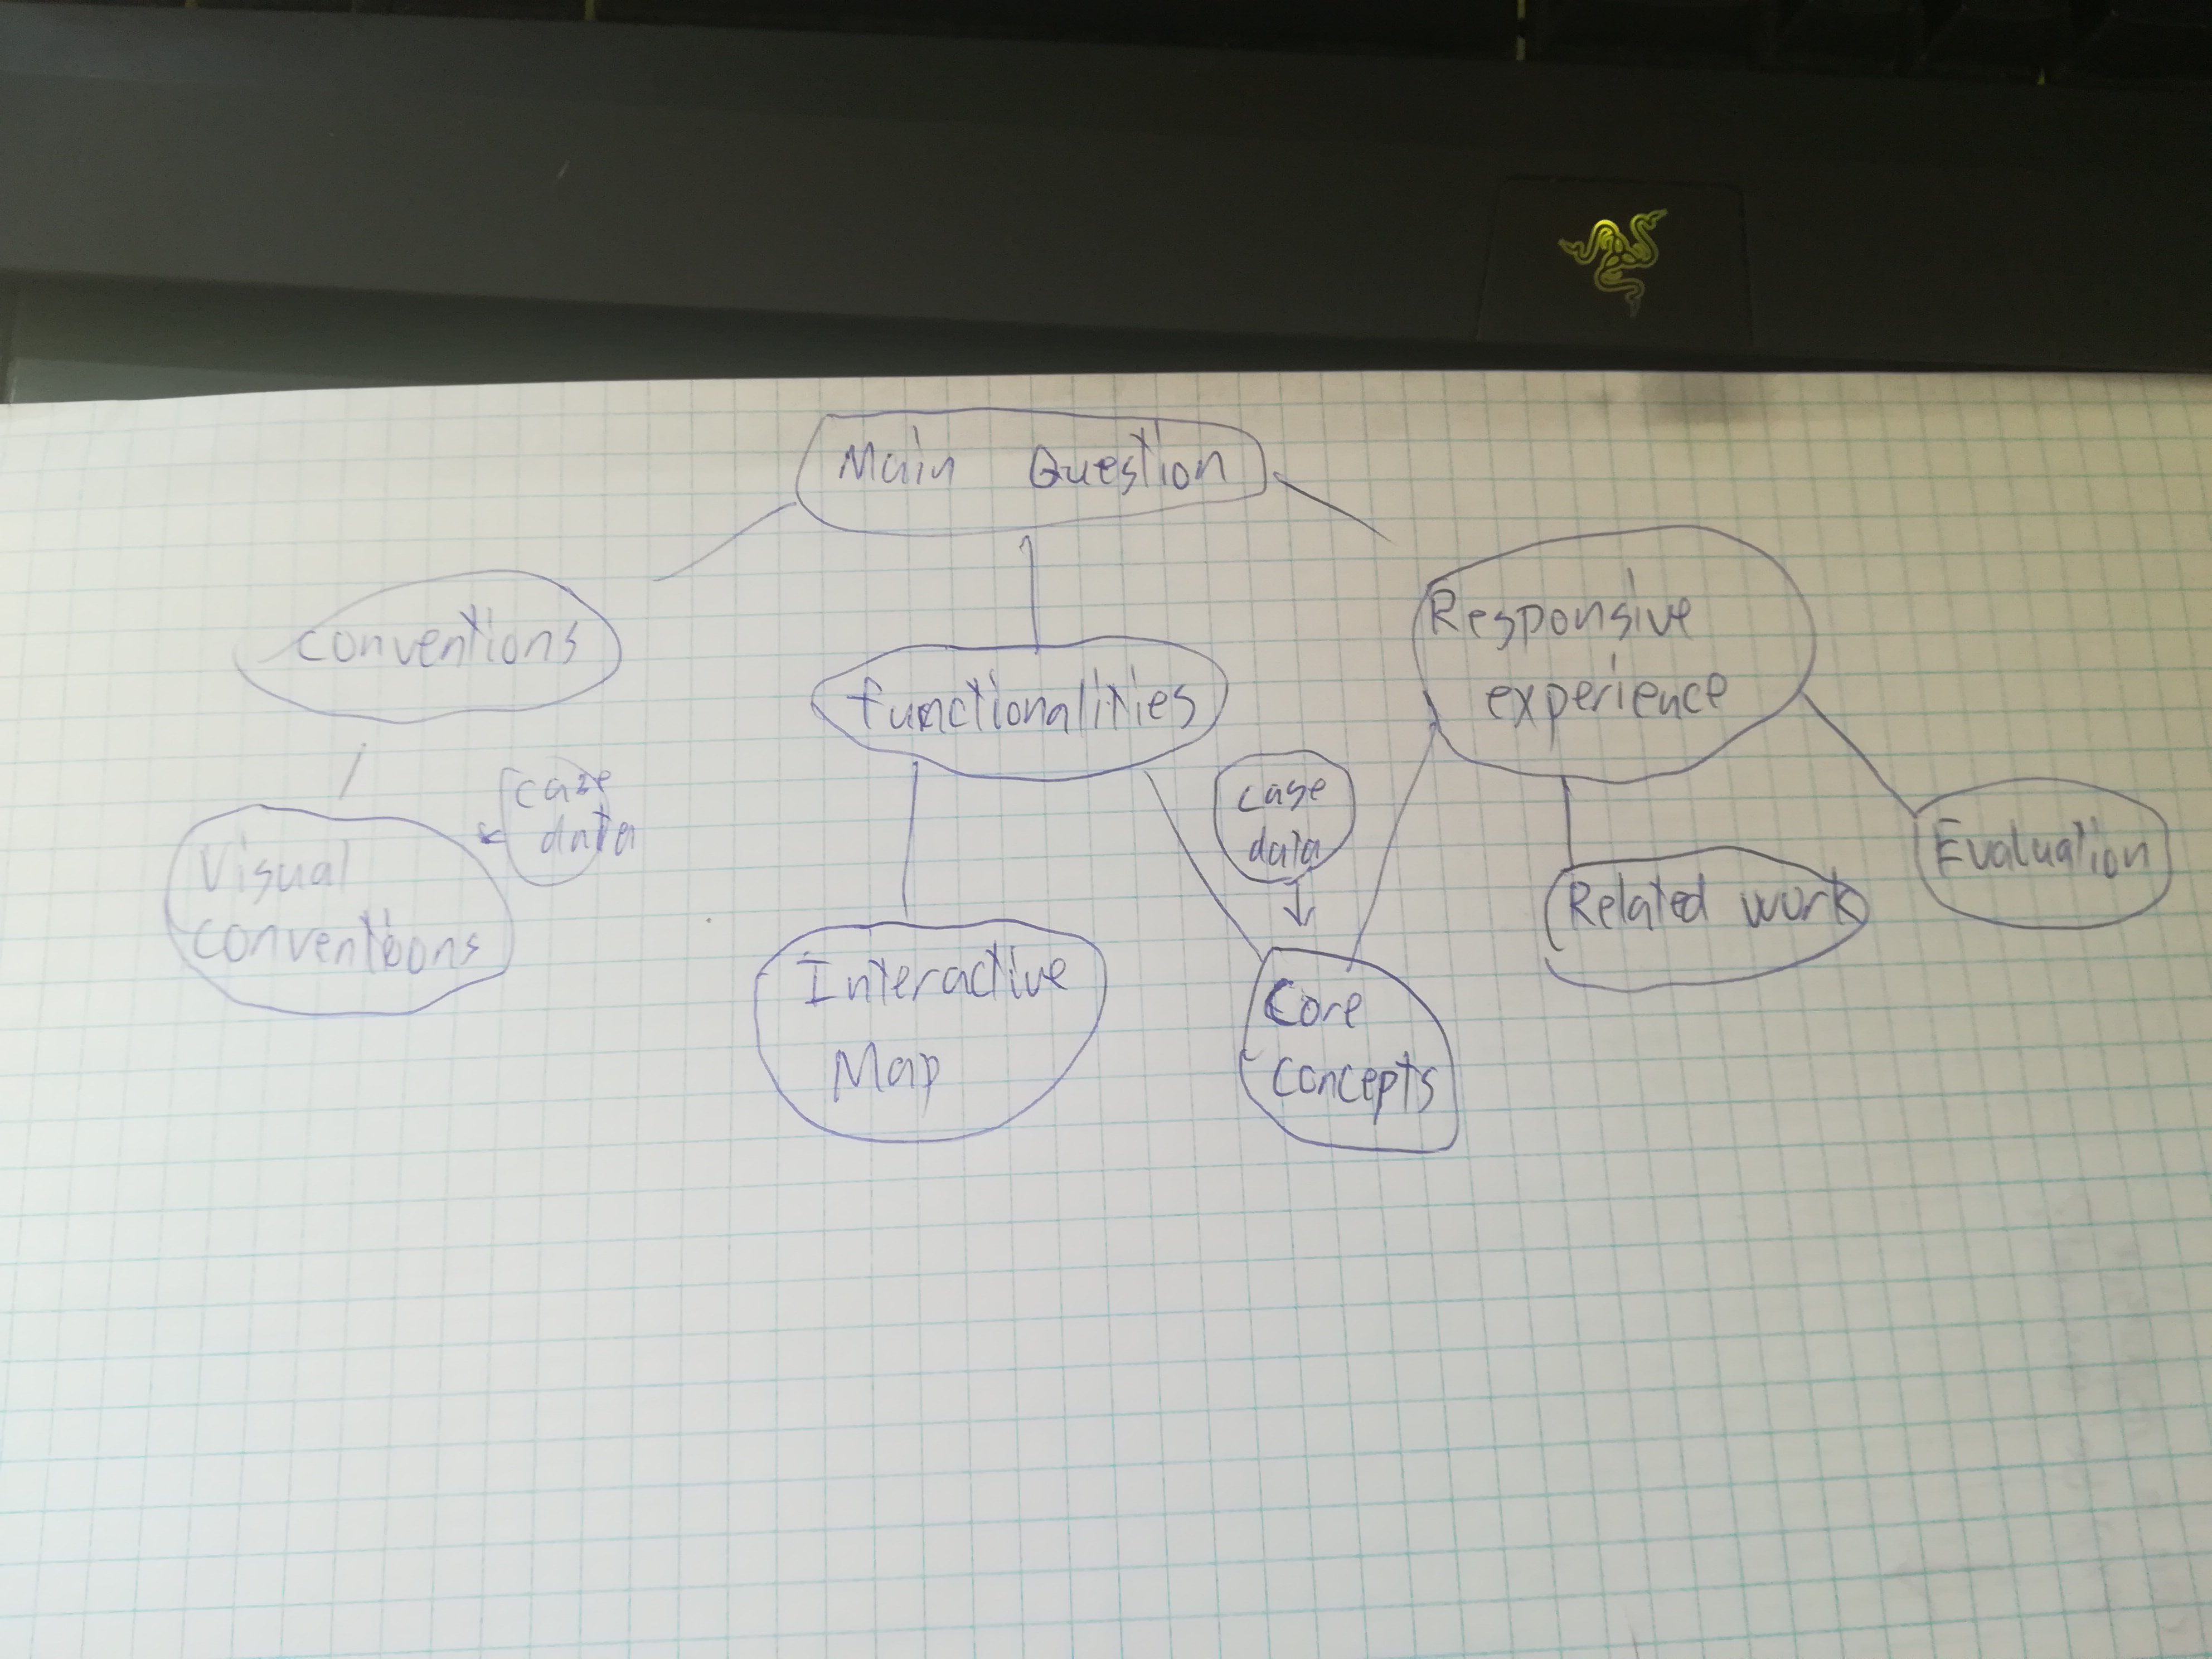
\includegraphics[width=.8\textwidth]{Pictures/Structure}
	\caption{Overview of how the research question gets answered in the first part of the report}
	\label{Structure}
\end{figure}

The rest of the first part is focused on answering the subquestions as illustrated in figure \ref{Structure}. 
The first subquestion is answered through a literature review in chapter x. After the visual conventions have been explained an example of an interactive map gets analysed in chapter x. This is done to understand which functionalities are important for such a map. This is followed by a review of related work in chapter x. Based on the related work and an initial exploration of the data five core concepts for the tool are created. These are described in chapter x. All of the considerations presented in this part then gets collected into the design in chapter x. 

The second part is the development of the tool. In chapter x the building blocks, which the tool is build from, are presented. How these building blocks are put together is then explained in chapter x. Chapter x is an overview of the final product.


The last part starts with an evaluation of the developed tool in chapter x. This is followed by chapter x with a discussion of the tool and how it could be developed further. The last chapter is the conclusion in chapter x 


\fxnote{Add a section, which summerieses the first part}

% \chapter{Examples}

\section{Figures}



\begin{figure} [H]
	\centering
	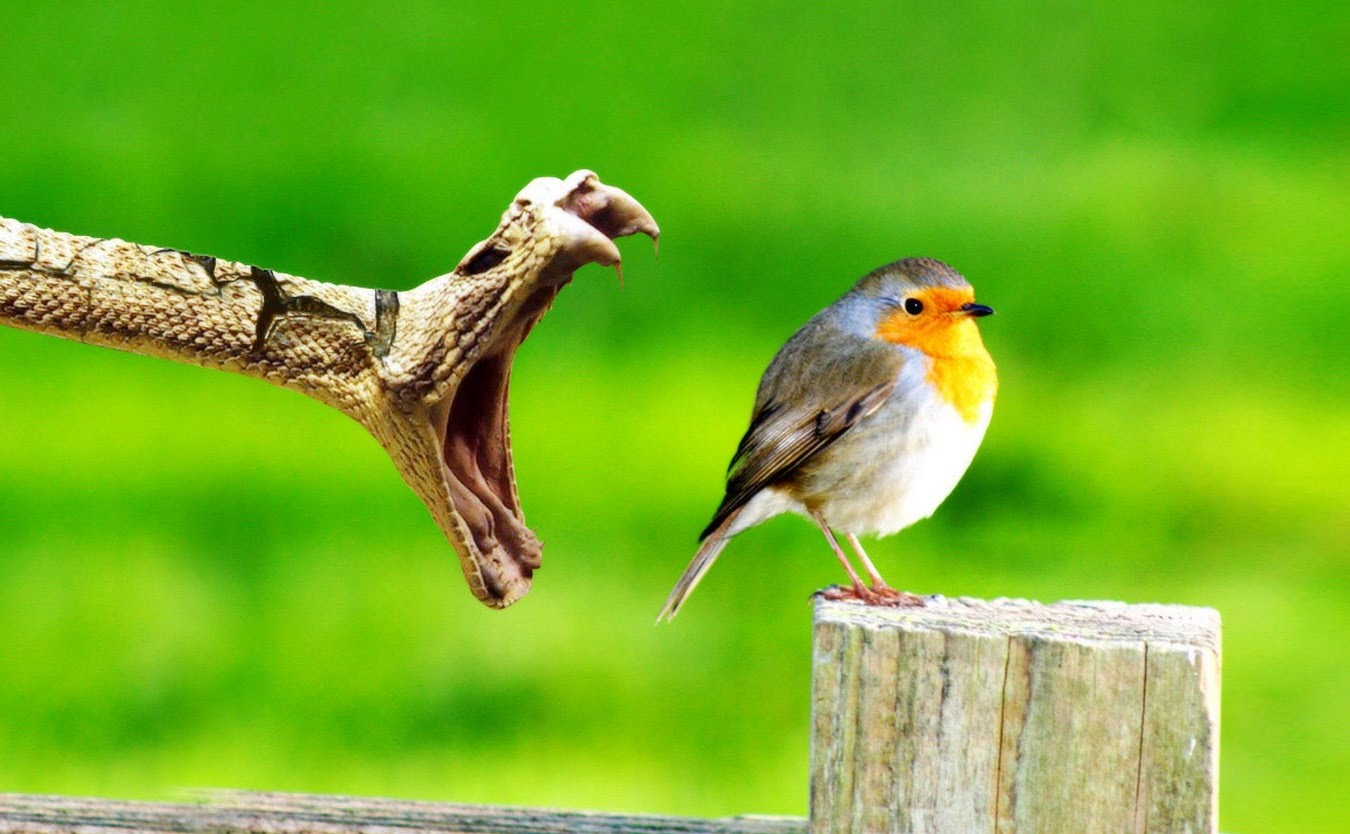
\includegraphics[width=.6\textwidth]{Pictures/Example.jpg}	
	\caption{This is a picture. Source: \citet{isover}}
	\label{Bird}
\end{figure}


\begin{figure} [H]
	\centering
	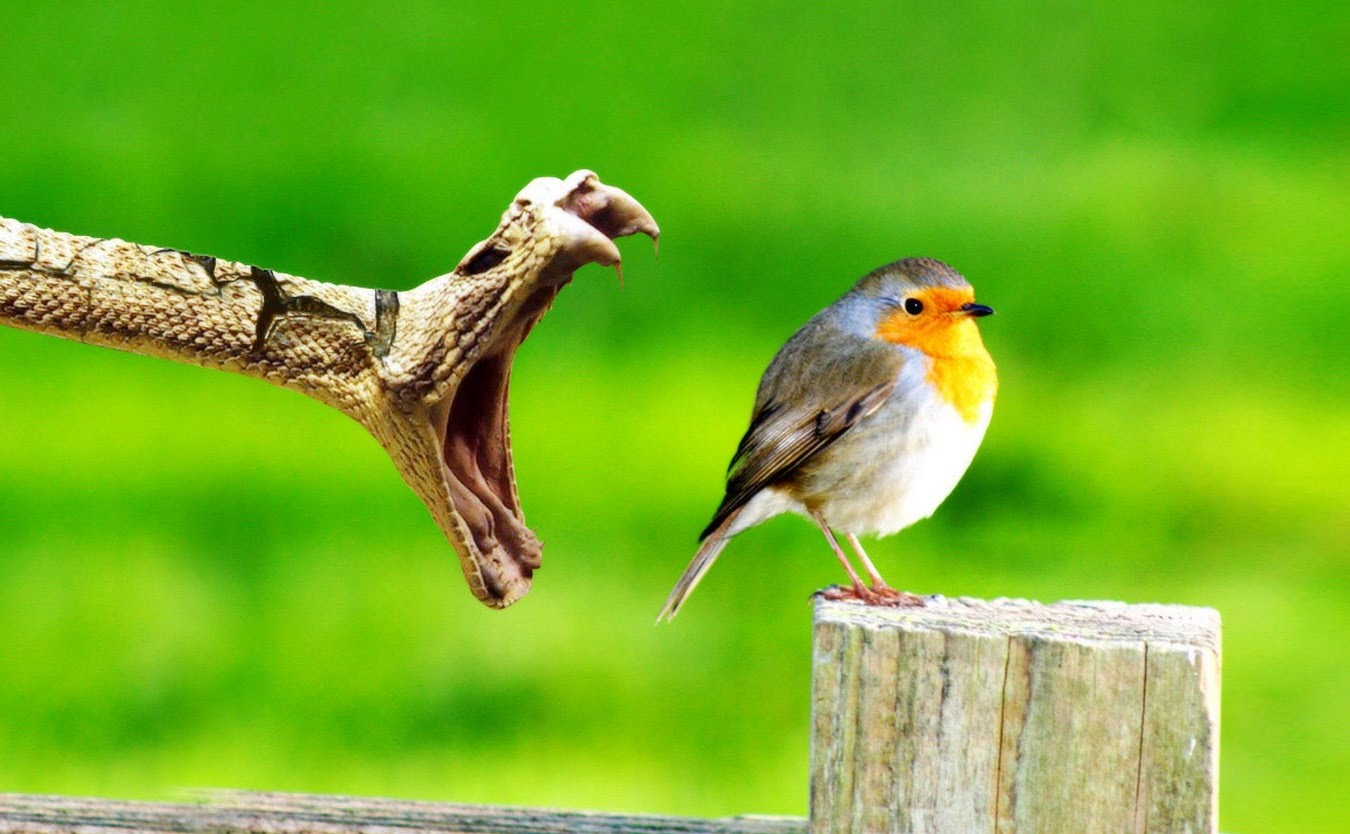
\includegraphics[width=.6\textwidth, angle=-90]{Pictures/Example.jpg}	
	\caption{This picture has been turned}
	\label{BirdTurned}
\end{figure}


\textbf{Cutting a picture}

\begin{figure} [H]
	\centering
	% trim={<left> <lower> <right> <upper>}
    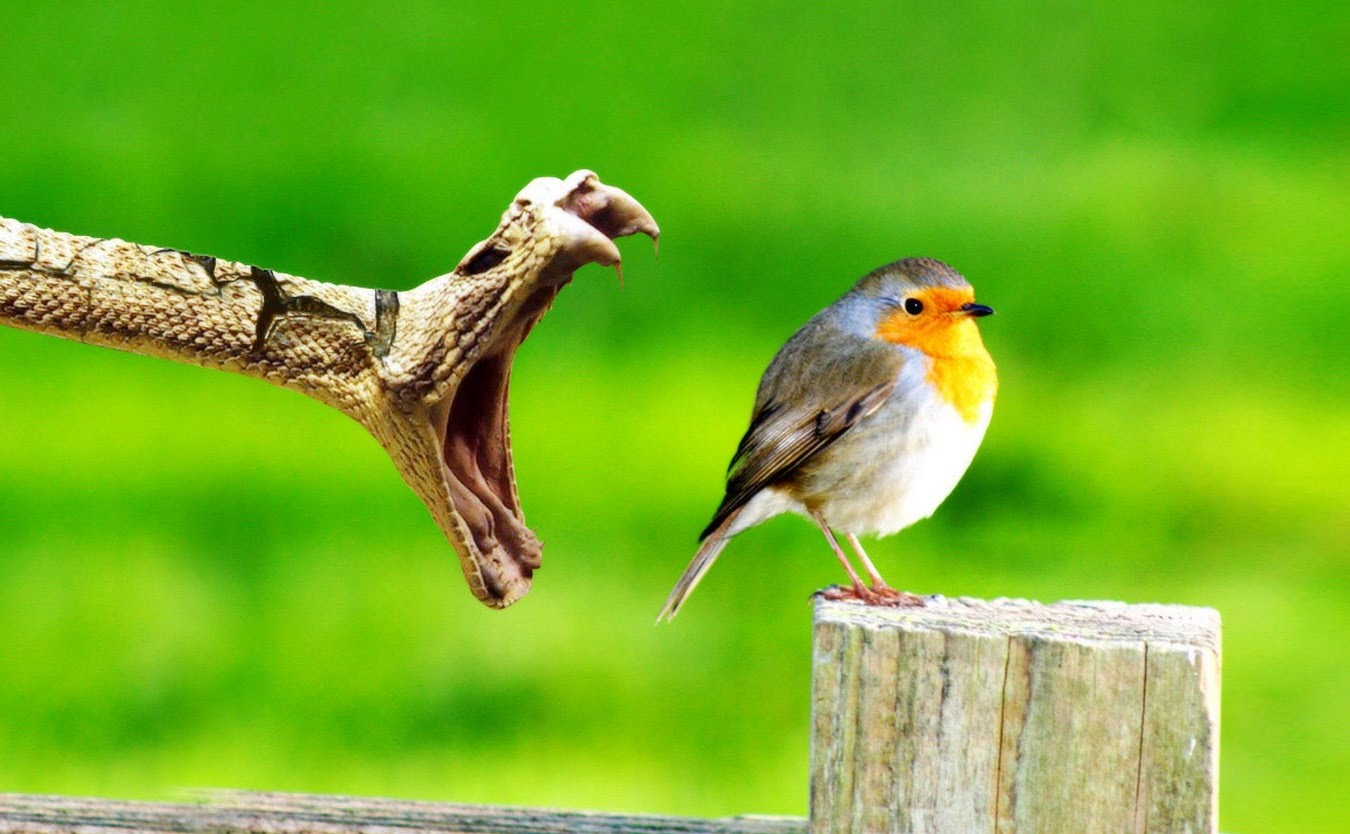
\includegraphics[width=.5\textwidth, trim={23cm 0 0 0},clip]{Pictures/Example.jpg}
	\caption{This picture has been cut}
	\label{BirdCut}
\end{figure}


Referencing to a particular figure is done like this:



\subsection{The Minipage}

\begin{figure} [h]
\begin{minipage}[t]{0.45\textwidth}
\centering
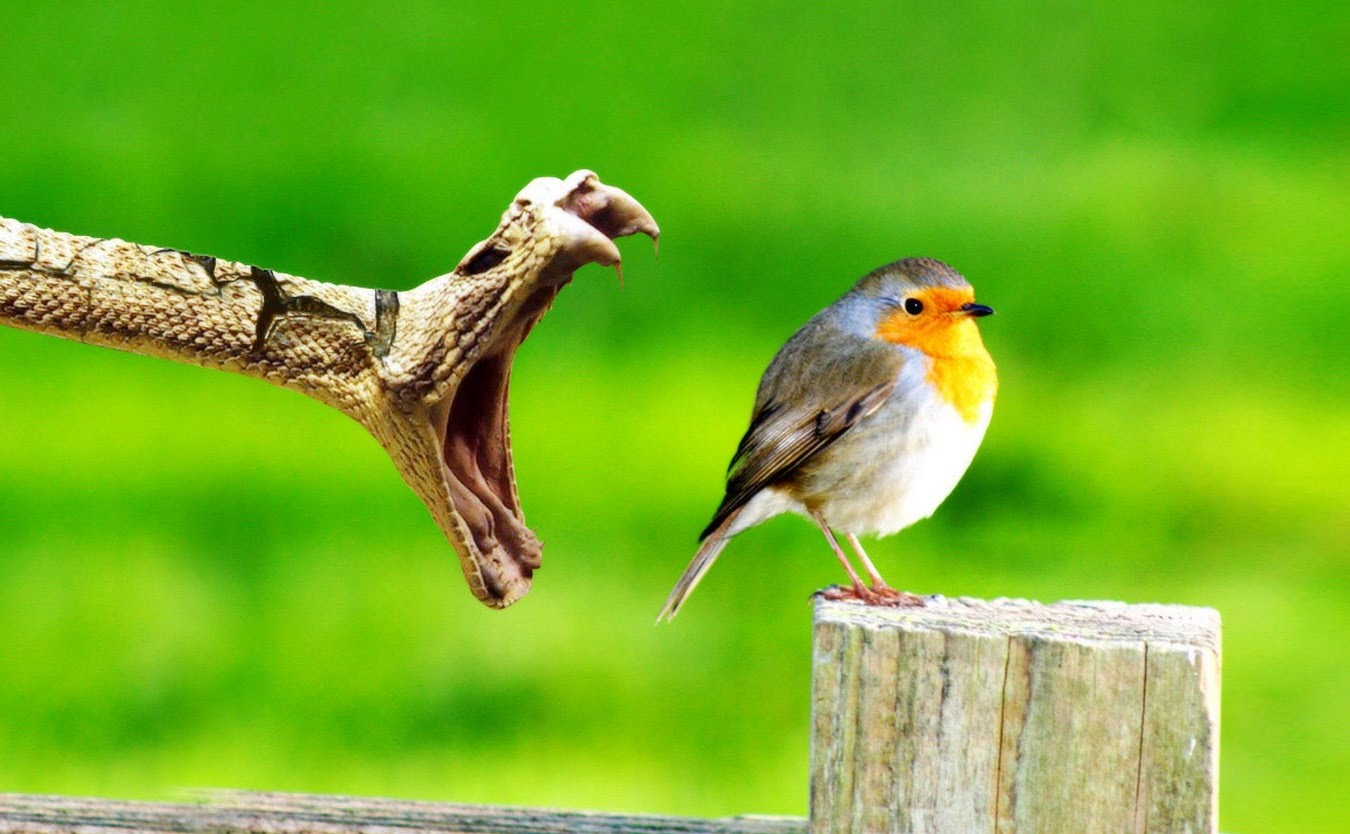
\includegraphics[width=1\textwidth]{Pictures/Example.jpg}
\caption{There is the same picture again}
\label{Bird2}
\end{minipage}
\hspace{0.1\textwidth}
\begin{minipage}[t]{0.45\textwidth}
\centering
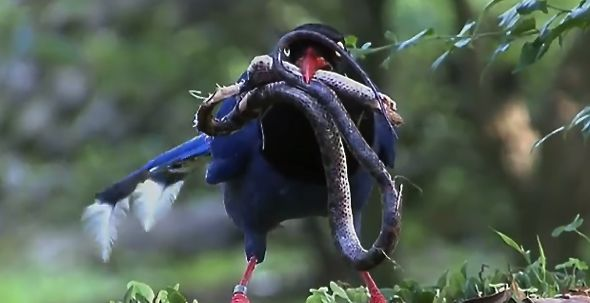
\includegraphics[width=1\textwidth]{Pictures/Example2.jpg}
\caption{Here is another picture.}
\label{Bird3}
\end{minipage}
\end{figure}

Sizes can be adjusted using this part: %\begin{minipage}[t]{0.3\textwidth}

\begin{figure} [h]
\begin{minipage}[t]{0.6\textwidth}
\centering
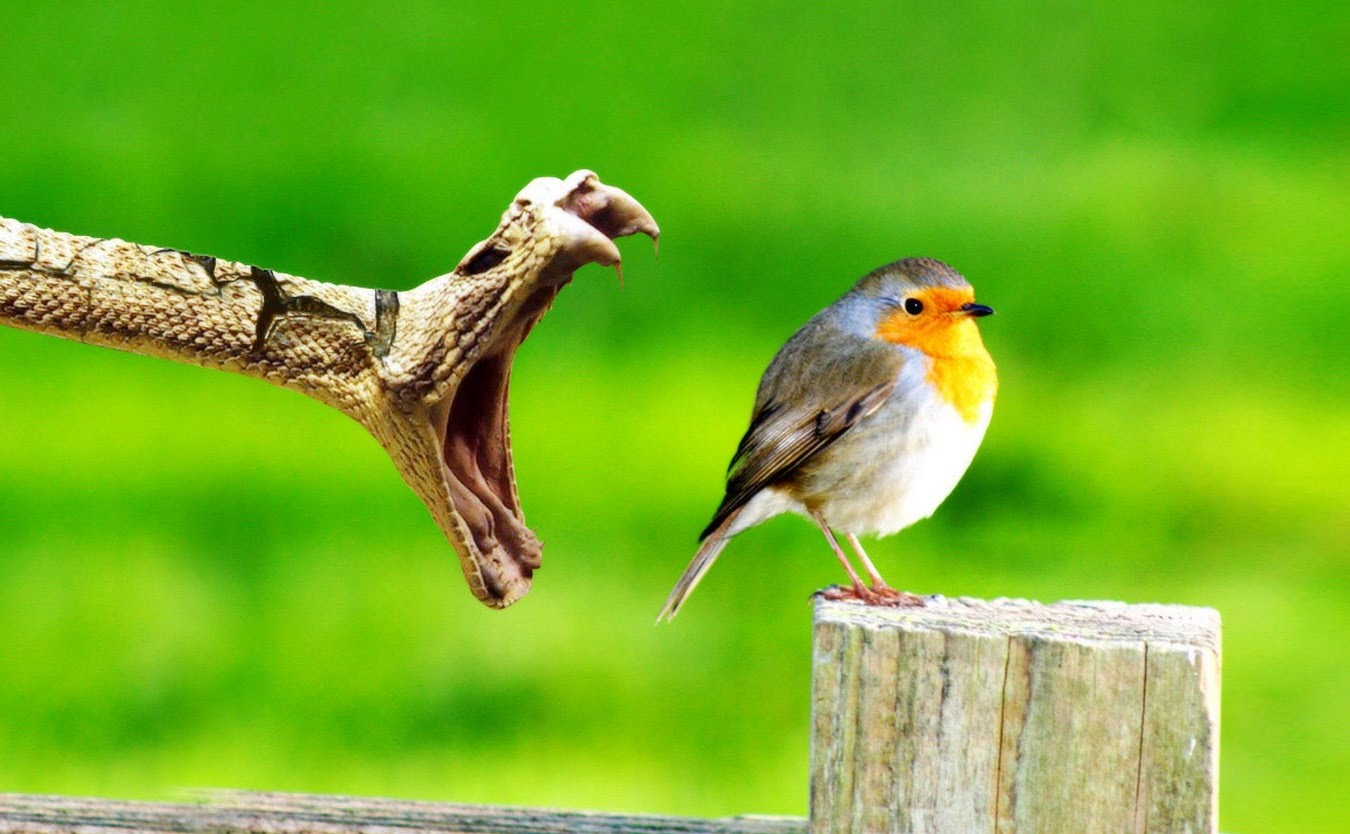
\includegraphics[width=1\textwidth]{Pictures/Example.jpg}
\caption{There is the same picture again}
\label{Bird4}
\end{minipage}
\hspace{0.05\textwidth}
\begin{minipage}[t]{0.3\textwidth}
\centering
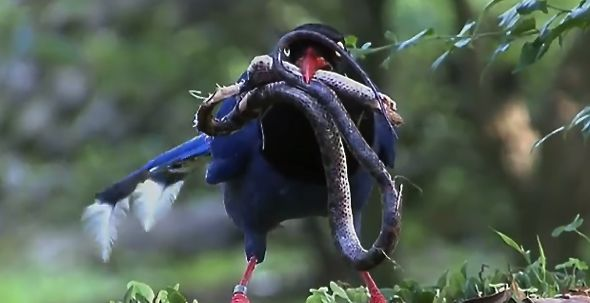
\includegraphics[width=1\textwidth]{Pictures/Example2.jpg}
\caption{Here is another picture. Source: \citet{isover}}
\label{Bird5}
\end{minipage}
\end{figure}







Making references to pictures are done by 
% \section{Tabulars}

\subsection{Real tabulars}

here are some text

\begin{table}[h]%You have to add this h yourself
\centering
\begin{tabular}{|c|cc|}
\hline
\multicolumn{2}{|c|}{Item}                   & \multicolumn{1}{r|}{} \\ \hline
Animal    & \multicolumn{1}{c|}{Description} & Price (\$)            \\ \hline
Gnat      & \multicolumn{1}{c|}{Frozen}      & 13.65                 \\ \hline
Gnu       & \multicolumn{1}{c|}{Stuffed}     & 92.50                 \\ \hline
Emu       & \multicolumn{1}{c|}{Stuffed}     & 33.33                 \\ \hline
Armadillo & \multicolumn{1}{c|}{Frozen}      & 8.99                  \\ \hline
\end{tabular}
\caption{This a real tabular}
\label{my-label}
\end{table}

also here

\subsection{Fake tabulars}



\begin{table}[htbp]
  \centering
    \begin{tabular}{l}
    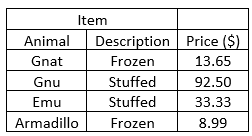
\includegraphics[width=0.5\textwidth]{Pictures/Tab}
    \end{tabular}%
  \caption{Add caption}
  \label{tab:addlabel}%
\end{table}%




%%%% Kilder %%%%

\begingroup
	\raggedright
	\bibliography{bibtex/litteratur}
	\endgroup	  % Litteraturlisten inkluderes



%%%% Appendiks %%%%

\appendix														% Appendiks/bilag start - giver chapter bogstaver i stedet for tal
\clearforchapter												% Sikrer at pagestylen aktiveres paa den rigtige side
\phantomsection													% Kunstigt afsnit, som hyperlinks kan 'holde fast i'
\pdfbookmark[0]{Appendiks}{appendiks}							% Tildeler en klikbar bookmark til den endelige PDF


% Indstillinger for appendiks (deaktiveret med "%") %%

\pagestyle{empty}												% Sidehoved/-fod for standardsider aendres til tom for appendiks
\aliaspagestyle{chapter}{empty}								% Sidehoved/-fod for kapitelsider aendres til tom for appendiks
\settocdepth{chapter}											% Kun kapitel-niveau vises i ToC
%\addtocontents{toc}{\protect\cftpagenumbersoff{chapter}}		% Sidetal for kapitler fjernes i ToC

% Filer til appendiks %%

\chapter{Lighthouse audit}\label{Audit}


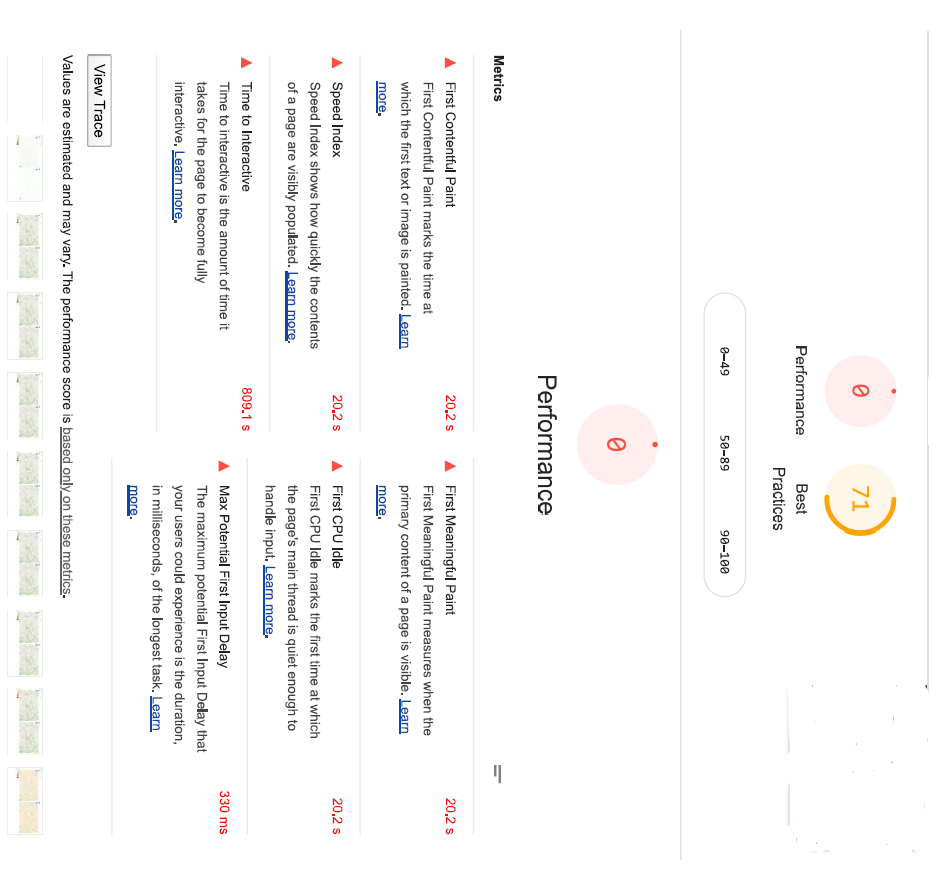
\includegraphics[width=1.2\textwidth, angle=90]{Pictures/Audit1}

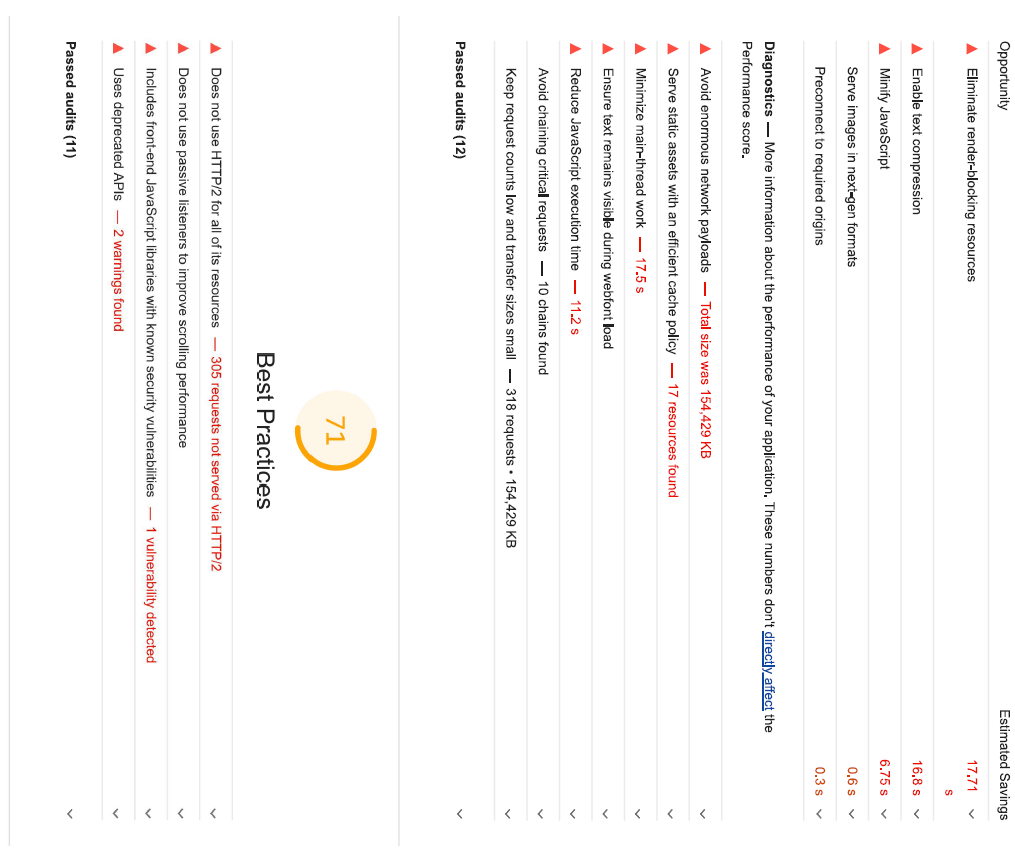
\includegraphics[width=1.2\textwidth, angle=90]{Pictures/Audit2}

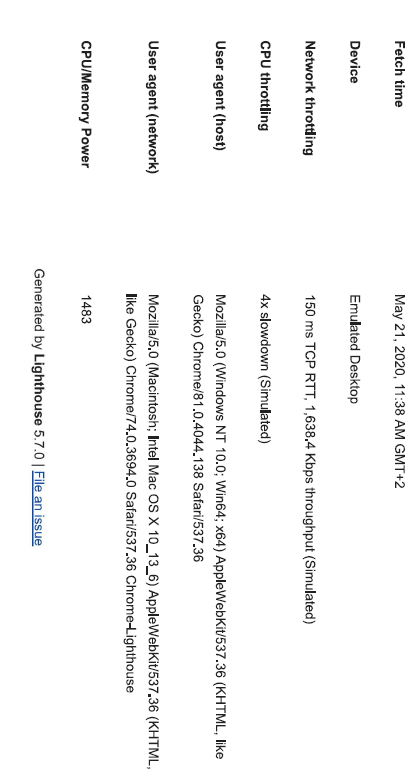
\includegraphics[width=0.6\textwidth, angle=90]{Pictures/Audit3}




%Flyt nederst

%%%% Bilag %%%%

%\phantomsection												% Kunstigt afsnit, som hyperlinks kan 'holde fast i'
%\addcontentsline{toc}{chapter}{Bilag A \ Navn} 				% Manuelle indgange i indholdsfortegnelsen (naar \includepdf bruges)
%\cleardoublepage
% Inkluder eksterne bilag med \includepdf[pages={x-y}]{filnavn}


%%%% Fixme-listen %%%%

\newpage														% Ny side til Fixme-listen
\listoffixmes													% Fixme-listen - fjernes til sidst i projektet med "%"



\end{document}													% % Slutter dokumentet - obligatorisk